%%%%%%%%%%%%%%%%%%%%%%%%%%%%%%%%%%%%%%%%%%%%%%%%%%%%%%%%%%%%%

\mainmatter
\setcounter{page}{1}

\lectureseries[\course]{\course}

\auth[\lecAuth]{Lecturer: \lecAuth\\ Scribe: \scribe}
\date{September 24, 2009}

\setaddress

% the following hack starts the lecture numbering at 9
\setcounter{lecture}{8}
\setcounter{chapter}{8}

\lecture{Least Squares Extensions}

\section{Least Squares Summary}
Up to this point we have seen that for a model
\begin{align}
\label{eq:09model}
\mathcal{M}: y(t) = \varphi^T(t)\theta + e(t,\theta)
\end{align}
we get the least squares estimate as
\begin{align}
\label{eq:lse}
\thn = \min_\theta\frac{1}{N}\sum_{t=1}^Ne^2(t,\theta)
\end{align}

\subsection{Properties of Least Squares Estimate}
These properties were all found in Lecture 8.

The expected value of the estimated parameter converges to the true parameter.
$$E\{\thn\} = \theta_0$$
provided the noise, $\{e(t)\}$, is white. This is for the system
\begin{align}
\label{eq:09sys}
\mathcal{S}: y(t) = \varphi^T(t)\theta_0 + e(t)
\end{align}

$R(N)$ and $f(N)$ are a collection of the auto-/cross-covariance functions.

The invertibility of $R(N)$ is equivalent to $\{u(t)\}$ being a persistently exciting signal.

\section{Variance Properties of Least Squares Estimate}
$$\text{cov}\{\thn\} = E\{(\thn-\theta_0)(\thn-\theta_0)^T\}$$
Converting the system in (\ref{eq:09sys}) to matrix form gives
\begin{align*}
\mathcal{S}: Y_N &= \Phi_N\theta_0+E_N \\
\Rightarrow \thn &= \left(\tfrac{1}{N}\Phi_N^T\Phi_N\right)^{-1}\left(\tfrac{1}{N}\Phi_N^TY_N\right) = R(N)^{-1}f(N)
\end{align*}
Then the covariance is found as
\begin{align*}
\text{cov}\{\thn\} &= E\left\lbrace\left(\tfrac{1}{N}\Phi_N^T\Phi_N\right)^{-1} \left(\frac{1}{N}\Phi_N^TE_N\right) \left(\tfrac{1}{N}E_N^T\Phi_N\right) \left(\tfrac{1}{N}\Phi_N^T\Phi_N\right)^{-1}\right\rbrace \\
&= \lambda E\left\lbrace\left(\tfrac{1}{N}\Phi_N^T\Phi_N\right)^{-1} \left(\tfrac{1}{N}\Phi_N^T\Phi_N\right) \left(\tfrac{1}{N}\Phi_N^T\Phi_N\right)^{-1}\right\rbrace \\
&\sim \lambda E\left\lbrace\left(\tfrac{1}{N}\Phi_N^T\Phi_N\right)^{-1}\right\rbrace
\end{align*}
where $\lambda = \frac{1}{N}E_NE_N^T$ is a scalar that can be moved outside the expectation operator. This shows that
$$\text{cov}\{\thn\} \sim \tfrac{1}{N}\lambda R^{-1}(N)$$
Hence we have that
$$\lim_{N\to\infty}\text{cov}\{\thn\} = 0$$
which makes $\thn$ a good estimator. The conclusion is
$$\lim_{N\to\infty}\thn = \theta_0 \text{ w.p. } 1$$
provided $u\perp e$, $\{e(t)\}$ is white noise $\Leftrightarrow \Phi\perp e$, $\mathcal{S}\in\mathcal{M} \Leftrightarrow \dim\theta = \dim\theta_0$ and that the regressor $\Phi(t)$ is known. When $\Phi(t)$ is known it means that the linearities and non-linearities of the system are known.

Often this type of least squares estimate is an academic exercise because do not \textit{really} know the parameter that describes the system.

It can be seen that $\frac{\lambda}{R(N)}$ is the noise-to-signal ratio. For a better estimate we need to take more measurements to increase $R(N)$.

The assumption that $\{e(t)\}$ is white noise means that we assume the dynamics of the noise and the system are the same. This rarely occurs in practice.

\section{Least Squares Extensions}
These are some ways that the least squares estimate can be modified to achieve better results in more general situations than those we have encountered so far. In other words, these extensions are methods used to overcome the limitations of the standard least squares estimator.

\subsection{Weighted Least Squares Estimate}
Starting with the model from (\ref{eq:09model}) and the estimate from (\ref{eq:lse}) we can add a weighting function such that
$$\thn = \min_\theta \frac{1}{N}\sum_{t=1}^N e_w^2(t)$$
where $e_w(t)=w(t)e(t)$. This can be useful for weighting recent data more than past data (Figure \ref{fig:09wRecent}) or for removing data that could be unreliable data (Figure \ref{fig:09bad}). The latter case allows us to ignore unreliable data that would result in determining a model that does not capture the dynamics of the actual system. The way to solve the weighted least squares problem is to find
$$\underbrace{w(t)y(t)}_{y_w(t)} = \underbrace{w(t)\varphi^T(t)}_{\varphi_w^T(t)}\theta + \underbrace{w(t)e(t)}_{e_w(t)}$$
and then use the standard tools. Note that this method can be used recursively.

\begin{figure}[ht!]
  \centering
  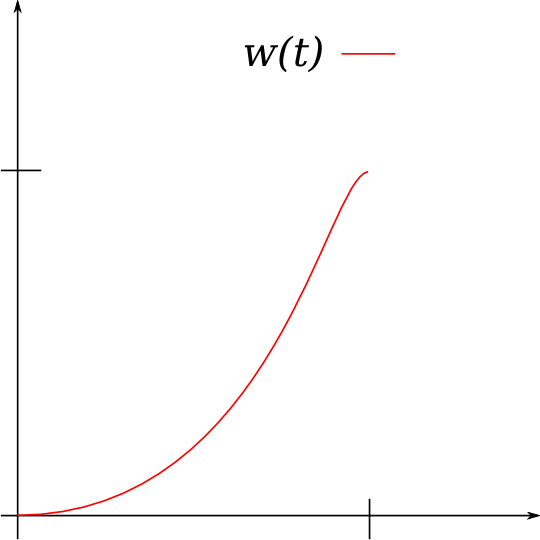
\includegraphics[width=.25\textwidth]{images/09wRecent}
  \caption{A weighting function to build an estimate using recent data more than past data.}
  \label{fig:09wRecent}
\end{figure}

\begin{figure}[ht!]
  \centering
  \subfloat[Data.]{
    \label{fig:09dataBad}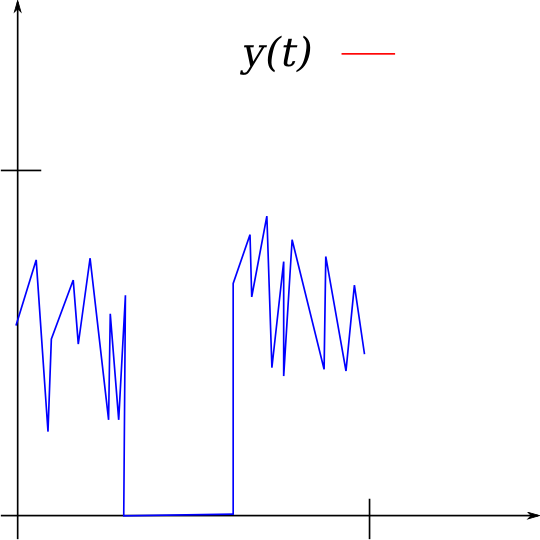
\includegraphics[width=0.3\textwidth]{images/09dataBad}
  } \hfill
  \subfloat[Weighting function.]{
    \label{fig:09wBad}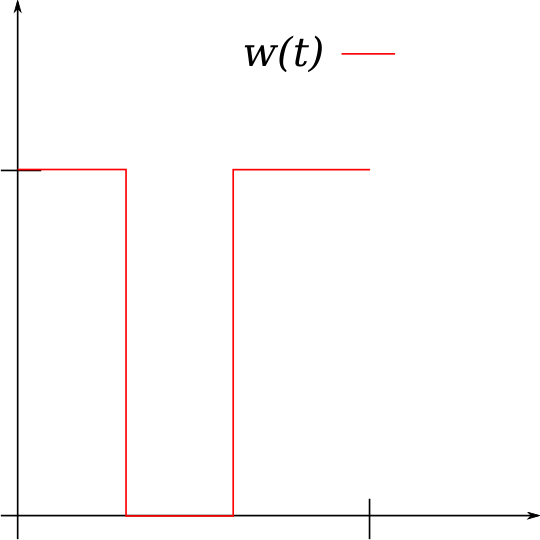
\includegraphics[width=0.3\textwidth]{images/09wBad}
  } \hfill
  \caption{Weighting function for unreliable data.}
  \label{fig:09bad}
\end{figure}

\subsection{Total Least Squares Estimate}
For this method we use a different model
$$\mathcal{M}: y(t) = (\varphi(t)+e_2(t,\theta))^T\theta+e_1(t,\theta)$$
This method minimizes the error on \textit{both} the input and the output, not just the output like the standard least squares estimate. See Figure \ref{fig:09totalLS}.

\begin{figure}[ht!]
  \centering
  \includegraphics[width=.3\textwidth]{images/09totalLS}
  \caption{Total least squares estimate uses inputs and outputs.}
  \label{fig:09totalLS}
\end{figure}

\subsection{Constrained Least Squares Estimate}
Suppose we have the model $\mathcal{M}: y(t) = \varphi^T(t)\theta + e(t,\theta)$ and having data $\{u(t),y(t)\}, t=1,\ldots,N$. Further suppose that we have a-priori knowledge of some part of the system dynamics that we want to use in our estimate. We then say that we will constrain the estimate so that it respects the a-priori knowledge of the system dynamics.

\begin{example}
Assume we know the DC-gain of $G_0(q)$. We can write the DC-gain of a system as being
\begin{align*}
G(q,\theta) &= \frac{b_0+b_1q^{-1}+\cdots+b_{n_b}q^{-n_b}}{1+a_1q^{-1}+\cdots+a_{n_a}q^{-n_a}} \\
\theta &= \left[\begin{array}{c c c c c c c} b_0 & b_1 & \cdots & b_{n_b} & a_1 & \cdots & a_{n_a} \end{array}\right]^T \\
\end{align*}
Then we look at the frequency response of the system to get $G(q,\theta)$. Taking the z-transform gives
$$G(q,\theta) \xrightarrow{q=z} G(z,\theta) \xrightarrow{z=e^{j\w}} G(e^{j\w},\theta)$$
If we substitute $q=1$ we get the DC-gain as
\begin{align}
\label{eq:constraint}
G_0(q) = \frac{b_0+b_1+\cdots+b_{n_b}}{1+a_1+\cdots+a_{n_a}} = s
\end{align}
where $s$ is a known scalar value. (\ref{eq:constraint}) is the constraint we wish to enforce. We can turn (\ref{eq:constraint}) into a linear constraint such that
\begin{align*}
&\frac{b_0+b_1+\cdots+b_{n_b}}{1+a_1+\cdots+a_{n_a}} = s \Leftrightarrow b_0+b_1+\cdots+b_{n_b} - s(1+a_1+\cdots+a_{n_a}) = 0 \\
&\Rightarrow \left[\begin{array}{c c c c c c c c c} 1 & 1 & \cdots & 1 & \vdots & -s & -s & \cdots & -s \end{array}\right]\theta-s=0 \\
&\Rightarrow A\theta = b
\end{align*}
where the second equation equals zero because $w(\theta)=0$ and the last equation shows the linear constraint as being $A\theta=b$. This results in the constrained least squares estimate being
$$\thn = \min_\theta\frac{1}{N}\sum_{t=1}^N\epsilon(t,\theta)$$
subject to $A\theta=b$. Next we find that
$$\hat{\theta}_N = \min_{\theta,\lambda}\left[\underbrace{\frac{1}{N}\sum_{t=1}^N\epsilon(t,\theta)}_{V(\theta)} +\lambda w(\theta)\right]$$
where $\lambda$ is called a constraint variable. To minimize this equation we must have
\begin{align*}
\frac{\partial\hat{\theta}_N}{\partial\theta}=0, \qquad \frac{\partial\hat{\theta}_N}{\partial\lambda}=0
\end{align*}
Recall that $\thn=R(N)^{-1}f(N)\Rightarrow R(N)\thn-f(N)=0$. Then we find
\begin{align*}
&\frac{\partial}{\partial\theta}V(\theta) +\lambda A = 0 \\
&\frac{\partial}{\partial\theta}V(\theta) = f(N)-R(N)\theta \\
&w(\theta)=0\rightarrow A^T\theta-b=0
\end{align*}
Also, because of the constraint we have that the error in the estimate is zero. Writing this out in matrix form yields
\begin{align*}
\underbrace{\left[\begin{array}{c c} R(N) & A \\ A^T & 0 \end{array}\right]}_{\tilde{R}_N} \left[\begin{array}{c} \hat{\theta} \\ \hat{\lambda} \end{array}\right] = \underbrace{\left[\begin{array}{c} f(N) \\ s \end{array}\right]}_{\tilde{f}_N}
\end{align*}
From this point we can just use the normal least squares method to get $\thn$ with the contraints built-in.
$\lozenge$
\end{example}

\section{Numerics and Computation}
\subsection{Left Inverse}
Consider the least squares problem in matrix form such that $Y=X\theta+E$. Writing this in matrix notation gives
$$\thn = \min_\theta E^TE = [X^TX]^{-1}[X^TY]$$
What does $[X^TX]^{-1}X^T$ represent? Looking at the dimensions of the matrices shows that
$$\underbrace{Y}_{N\times1} = \underbrace{X}_{N\times p} \underbrace{\theta}_{p\times1} + \underbrace{E}_{N\times1}$$
Since $X$ is not square we cannot take the inverse of it. However, we \textit{can} use
\begin{align}
\label{eq:li}
\underbrace{[X^TX]^{-1}X^T}_{p\times N} \cdot \underbrace{X}_{N\times p} = I
\end{align}
This shows that the term $[X^TX]^{-1}X^T$ is the \textit{left-inverse} of $X$ and is available to compute. To actually compute the left-inverse without calculating all of the inverses in (\ref{eq:li}) Householder transformations are normally used. In \textsc{Matlab} the command for the left-inverse of $X$ times $Y$ is done using \texttt{X\textbackslash Y}.

\subsection{Condition Number}
It can be seen that the left-inverse, $[X^TX]^{-1}X^T$, is dependent on the condition number of $X$ such that
$$\kappa(X^TX) = \kappa(X)^2$$
Singular values can be used to find the condition number of a matrix where
$$X\rightarrow \bar{\sigma}(X), \underline{\sigma}(X), \kappa(X)=\frac{\bar{\sigma}(X)}{\underline{\sigma}(X)}$$

\subsection{Proper Calculation of Least Squares}
This leads to the real way that a least squares estimate is found. Let $||\cdot||_F$ denote the Frobenius norm. Also, recall that a $QR$ factorization can be used to transform a matrix using $A=QR$, where $Q$ is orthonormal meaning $QQ^T=Q^TQ=I\rightarrow\kappa=1$ and $R$ is upper triangular. Then
\begin{align}
\min_\theta E^TE &= \min_\theta||E||_F \nonumber \\
&= \min_\theta||Y-X\theta||_F \nonumber \\
&= \min_\theta\vectornorm{\left[\begin{array}{c c} X & Y \end{array}\right] \left[\begin{array}{c} -\theta \\ I \end{array}\right]}_F \nonumber \\
&= \min_\theta\vectornorm{Q\left[\begin{array}{c c} R_{11} & R_{12} \\ 0 & R_{22} \end{array}\right] \left[\begin{array}{c} -\theta \\ I \end{array}\right]}_F \nonumber \\
&= \min_\theta\vectornorm{\left[\begin{array}{c c} R_{11} & R_{12} \\ 0 & R_{22} \end{array}\right] \left[\begin{array}{c} -\theta \\ I \end{array}\right]}_F \nonumber \\
&= \min_\theta\vectornorm{R_{12}-R_{11}\theta}_F + \vectornorm{R_{22}}_F \nonumber \\
\label{eq:lsreal}
\thn &= R_{11}^{-1}R_{12} \\
\label{eq:lserror}
\min_\theta E^TE &= \vectornorm{R_{22}}_F
\end{align}
(\ref{eq:lsreal}) and (\ref{eq:lserror}) are very important equations and show the proper way to compute a least squares estimate.

\subsection{Computer Precision}
On modern computer hardware running \textsc{Matlab} the machine precision is approximately $10^{15}$. If $\kappa(X)=10^7$ then $\kappa(X^TX)=10^{14}$ which is getting close to the hardware limit. However, using (\ref{eq:lsreal}) for the least squares estimate gives a condition number of $\kappa(X)=\kappa(R_{11})=10^7$. The difference between methods used for computing the least squares estimate can make the difference between whether a problem is computationally feasible or not.

%%%%%%%%%%%%%%%%%%%%%%%%%%%%%%%%%%%%%%%%%%%%%%%%%%%%%%%%%%%%%